\documentclass[class=NCU_thesis, crop=false]{standalone}
\usepackage[newfloat]{minted}
\usepackage{floatrow}
\usepackage{graphicx}


\begin{document}

\chapter{實驗設計與結果}

\section{實驗一:機械臂的基本控制}
\subsection{機械結構設計圖}
本實驗的硬體部分使用了3D列印技術,結合小型伺服馬達,設計了一個頂端為夾爪的小型機械臂,以下為此硬體的詳細設計圖紙:
\begin{figure}[htbp]
    \centering
    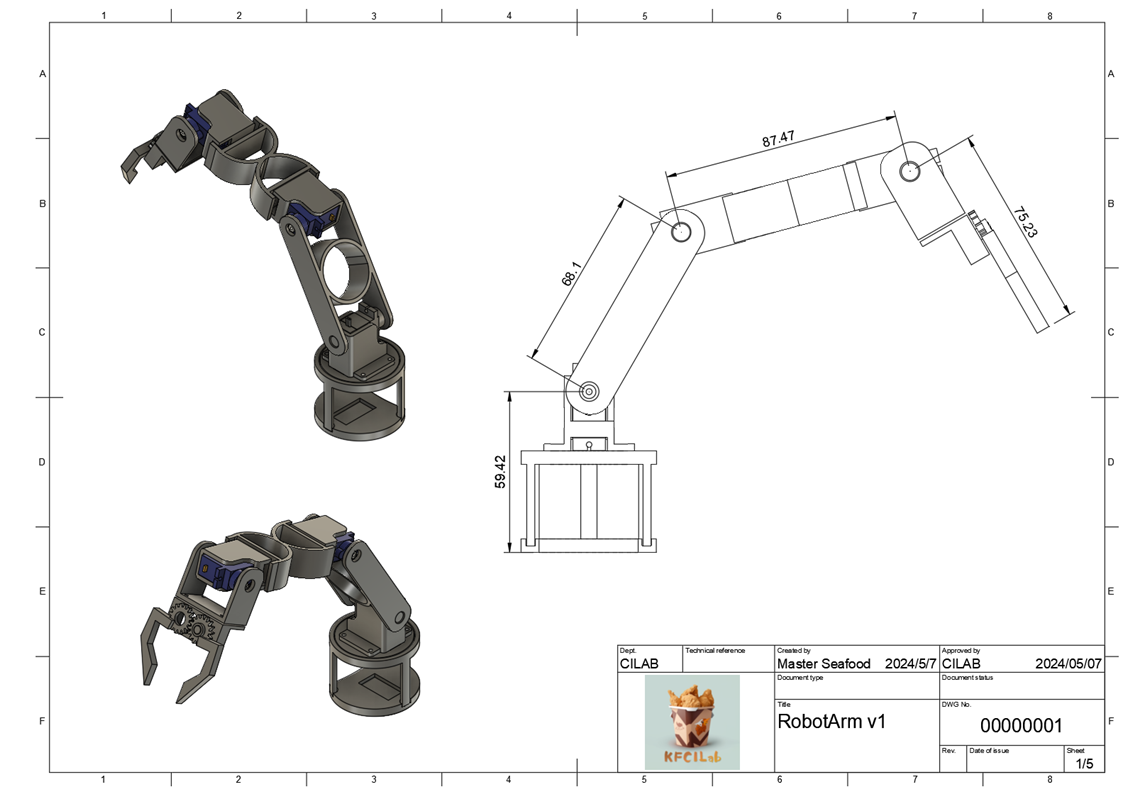
\includegraphics[width=0.9\textwidth]{figures/Armv1 (1).PNG}
    \caption{機械臂版本一設計圖紙 第一頁(單位:mm)}
    %\label{fig:Armv1Drawing_p1}}
\end{figure}

\begin{figure}[htbp]
    \centering
    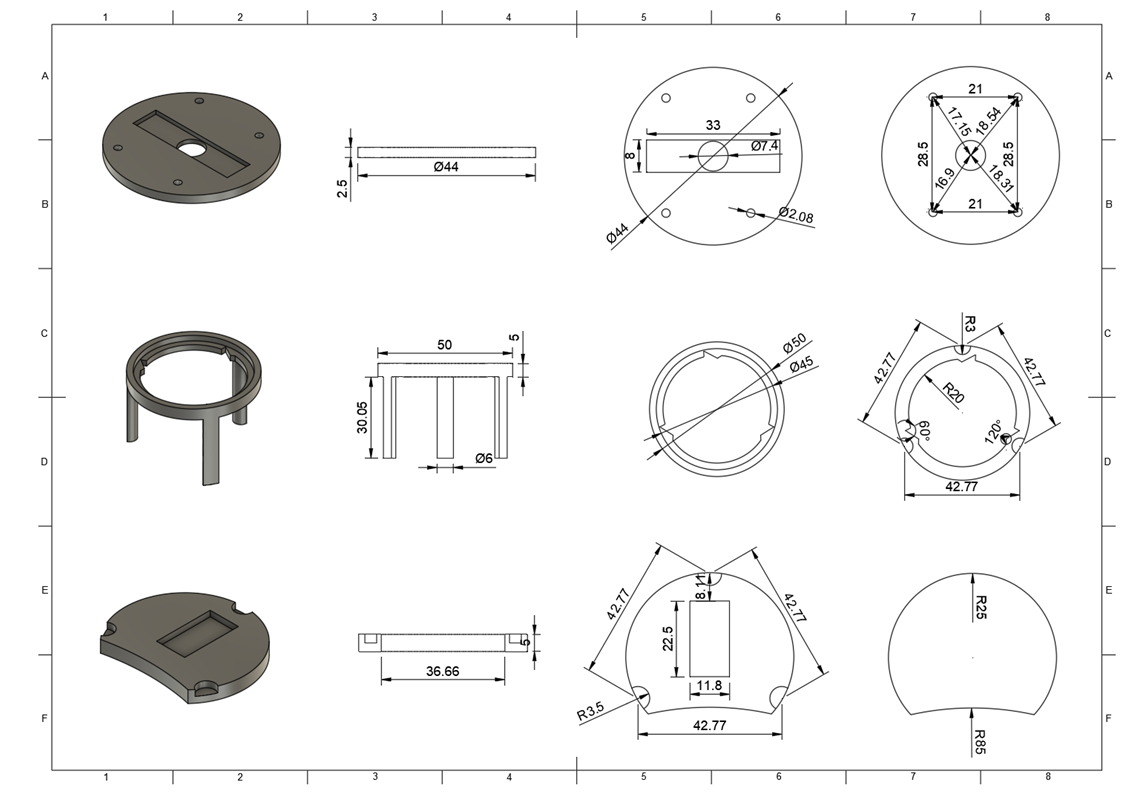
\includegraphics[width=0.9\textwidth]{figures/Armv1 (2).PNG}
    \caption{機械臂版本一設計圖紙 第二頁(單位:mm)}
\end{figure}

\begin{figure}[htbp]
    \centering
    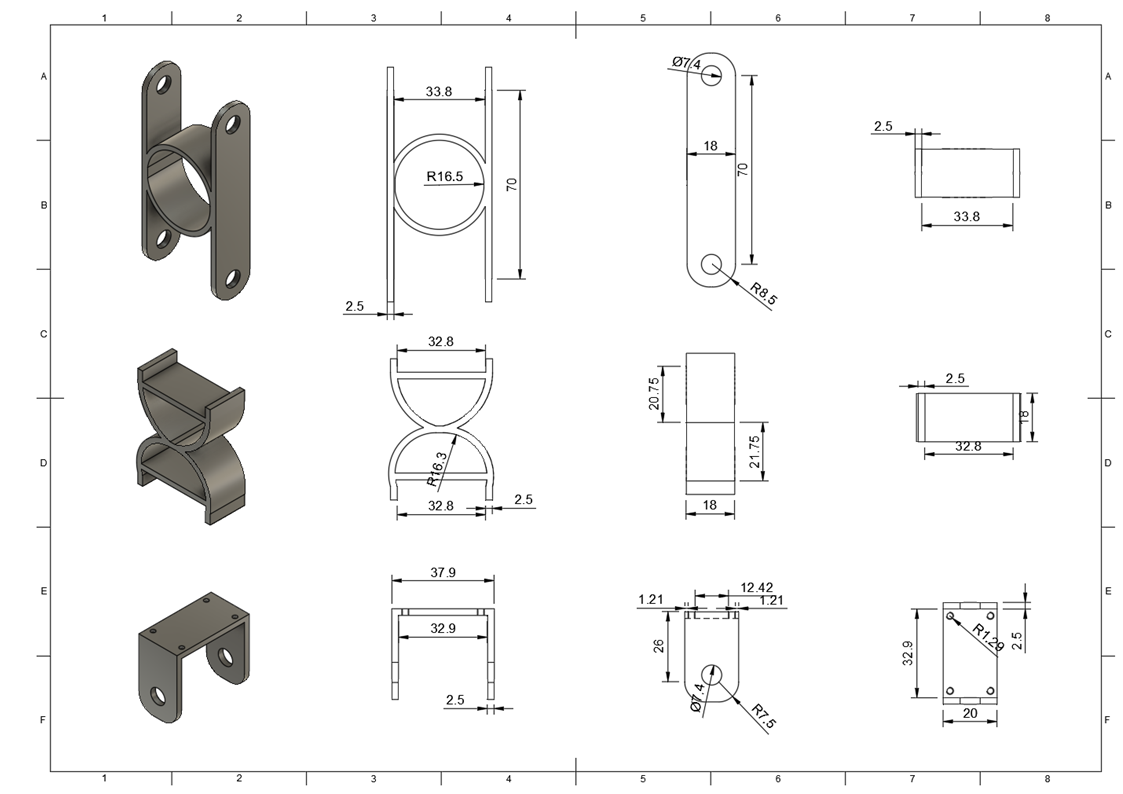
\includegraphics[width=0.9\textwidth]{figures/Armv1 (3).PNG}
    \caption{機械臂版本一設計圖紙 第三頁(單位:mm)}
\end{figure}

\begin{figure}[htbp]
    \centering
    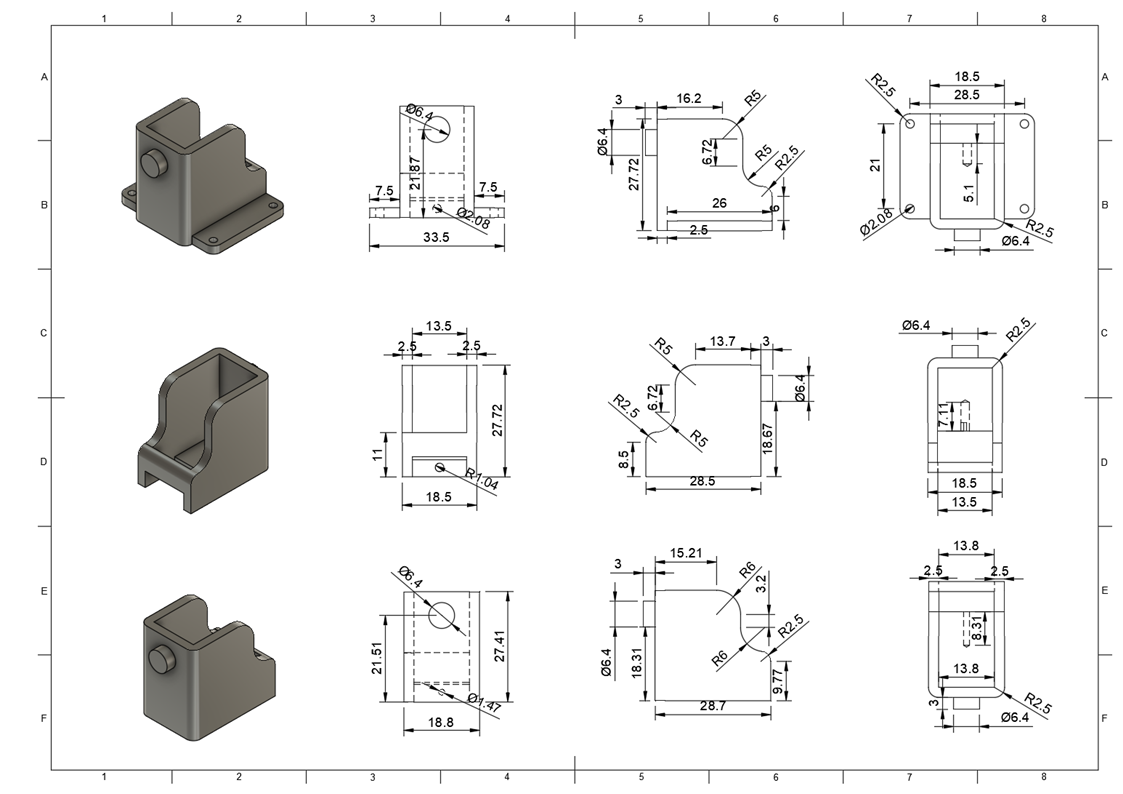
\includegraphics[width=0.9\textwidth]{figures/Armv1 (4).PNG}
    \caption{機械臂版本一設計圖紙 第四頁(單位:mm)}
\end{figure}

\begin{figure}[htbp]
    \centering
    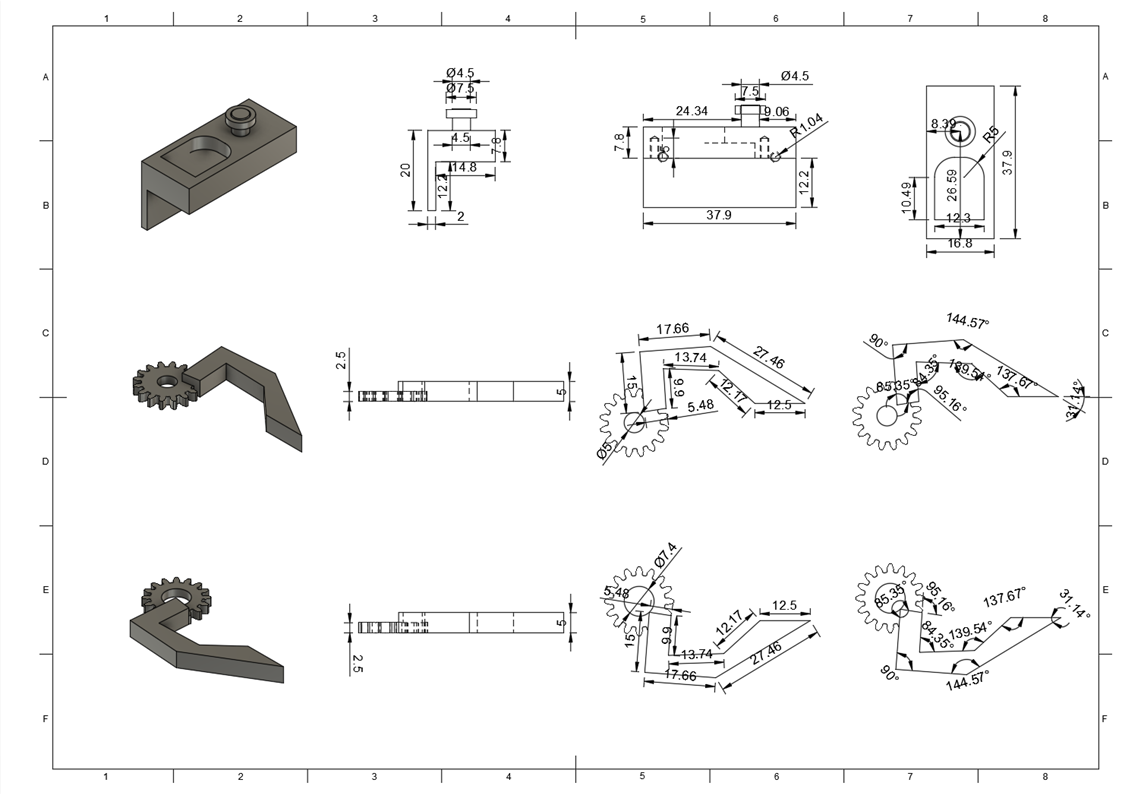
\includegraphics[width=0.9\textwidth]{figures/Armv1 (5).PNG}
    \caption{機械臂版本一設計圖紙 第五頁(單位:mm)}
\end{figure}



\section{實驗二:將機械臂用於畫圖}
\subsection{機械結構設計圖}
本實驗的硬體部分使用了3D列印技術,結合小型伺服馬達,設計了一個畫筆的小型機械臂,以下為此硬體的詳細設計圖紙:
\begin{figure}[htbp]
    \centering
    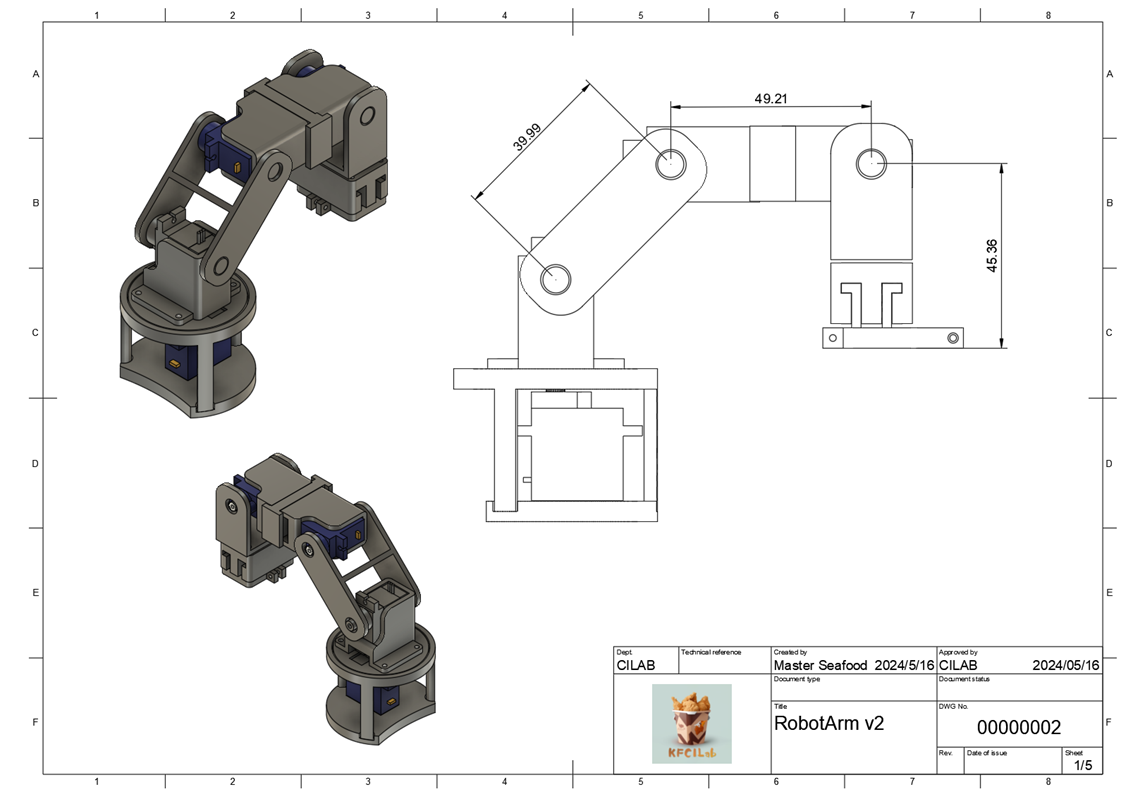
\includegraphics[width=0.9\textwidth]{figures/Armv2 (1).PNG}
    \caption{機械臂版本二設計圖紙 第一頁(單位:mm)}
    %\label{fig:Armv1Drawing_p1}}
\end{figure}

\begin{figure}[htbp]
    \centering
    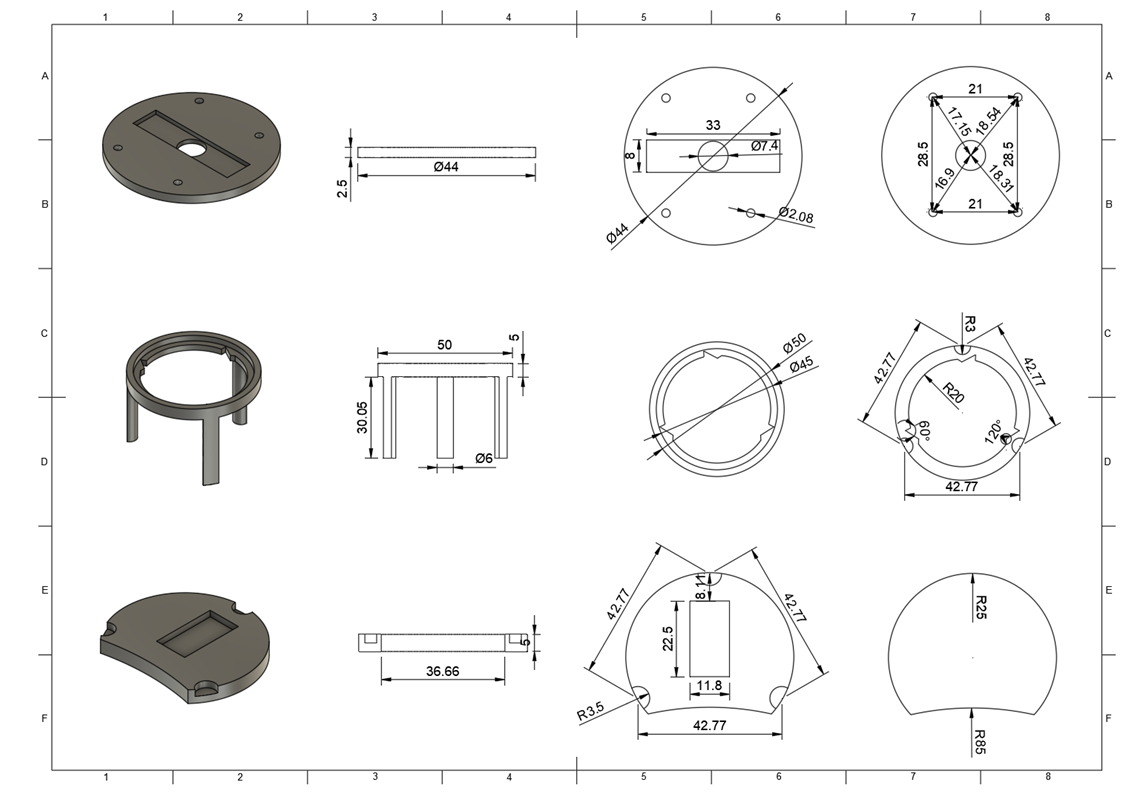
\includegraphics[width=0.9\textwidth]{figures/Armv2 (2).PNG}
    \caption{機械臂版本二設計圖紙 第二頁(單位:mm)}
\end{figure}

\begin{figure}[htbp]
    \centering
    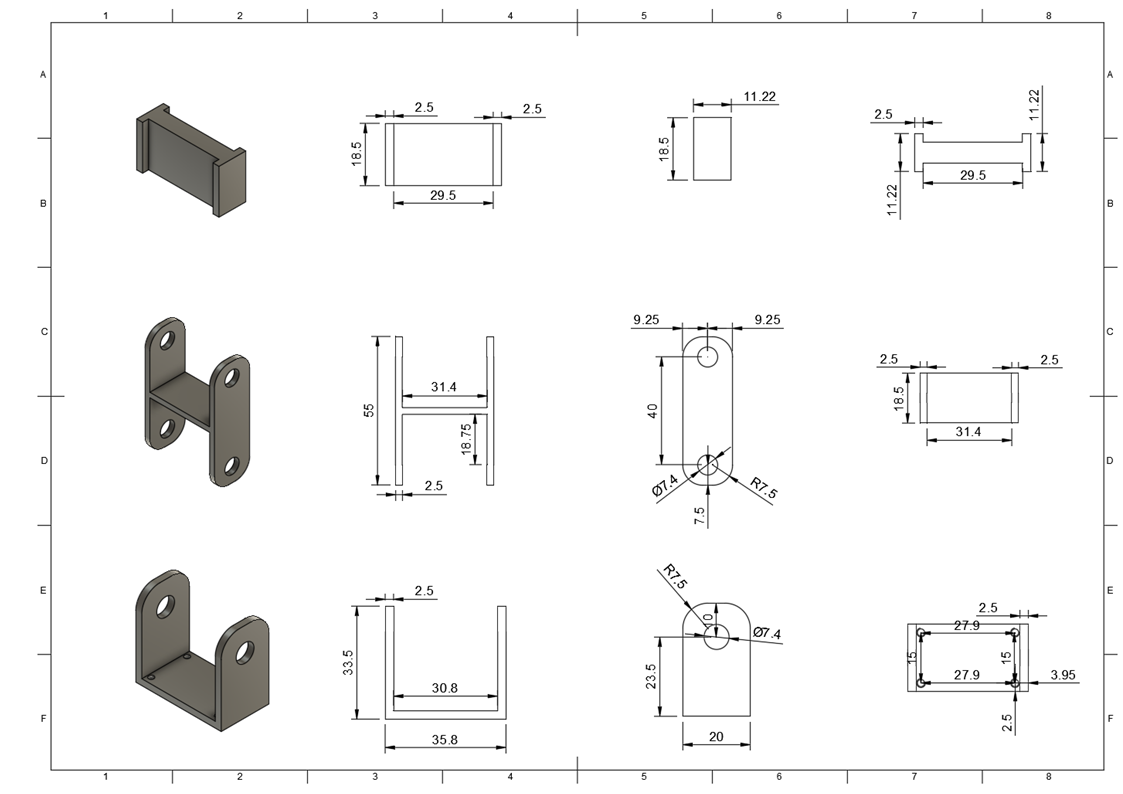
\includegraphics[width=0.9\textwidth]{figures/Armv2 (3).PNG}
    \caption{機械臂版本二設計圖紙 第三頁(單位:mm)}
\end{figure}

\begin{figure}[htbp]
    \centering
    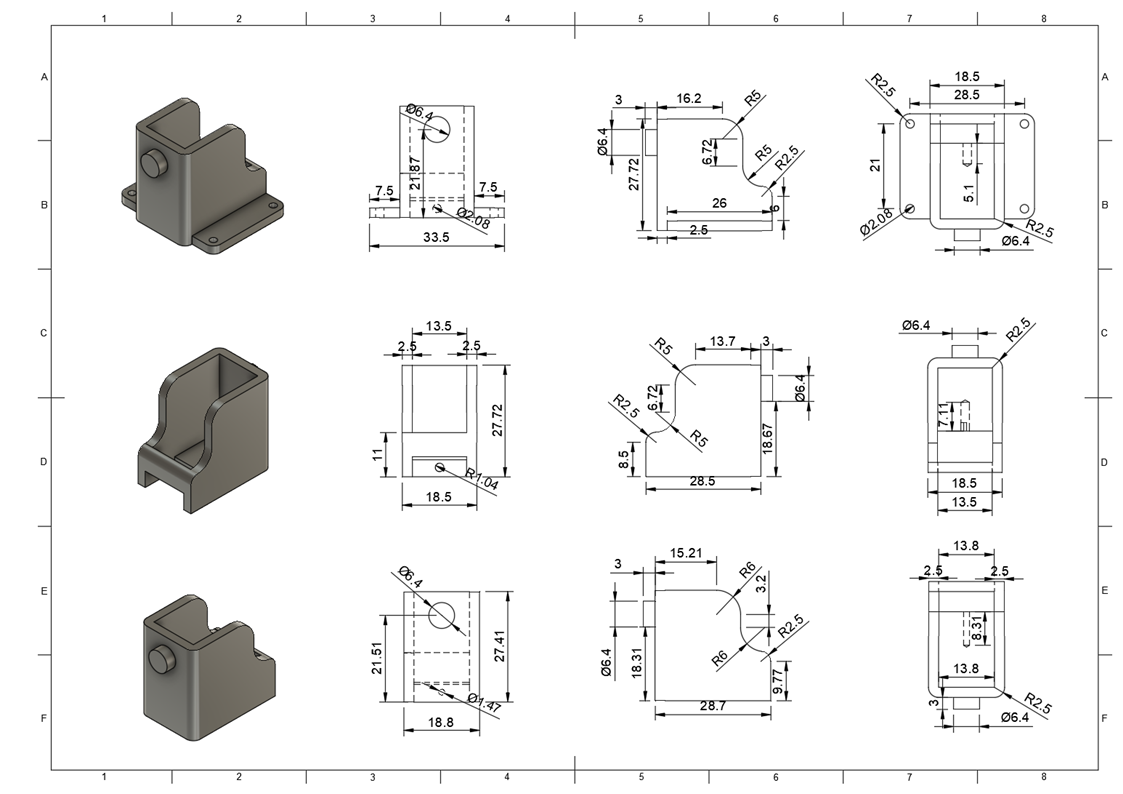
\includegraphics[width=0.9\textwidth]{figures/Armv2 (4).PNG}
    \caption{機械臂版本二設計圖紙 第四頁(單位:mm)}
\end{figure}

\begin{figure}[htbp]
    \centering
    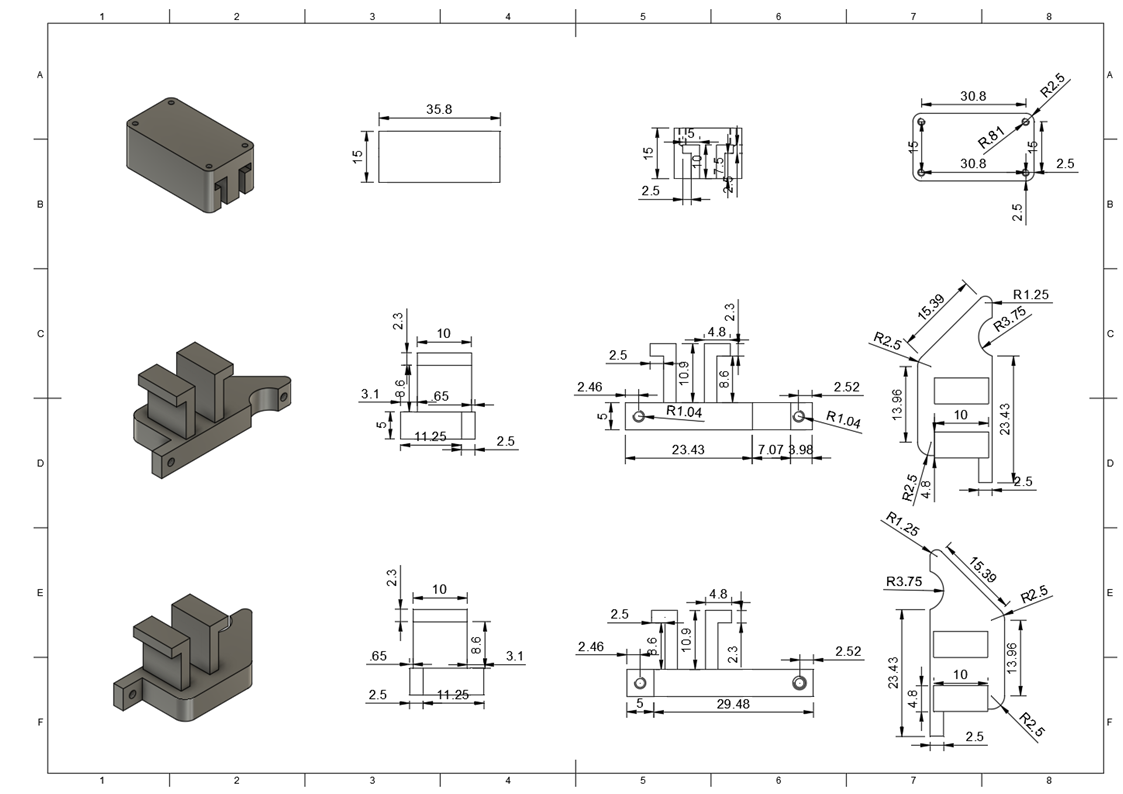
\includegraphics[width=0.9\textwidth]{figures/Armv2 (5).PNG}
    \caption{機械臂版本二設計圖紙 第五頁(單位:mm)}
\end{figure}

\section{實驗三:機械臂在自動運輸車上的應用}
\subsection{機械結構設計圖}
本實驗將機械臂與自動運輸車、鏡頭等硬體結合,設計了一台裝載機械臂的無人搬運車,以下為此硬體的詳細設計圖紙:
\begin{figure}[htbp]
    \centering
    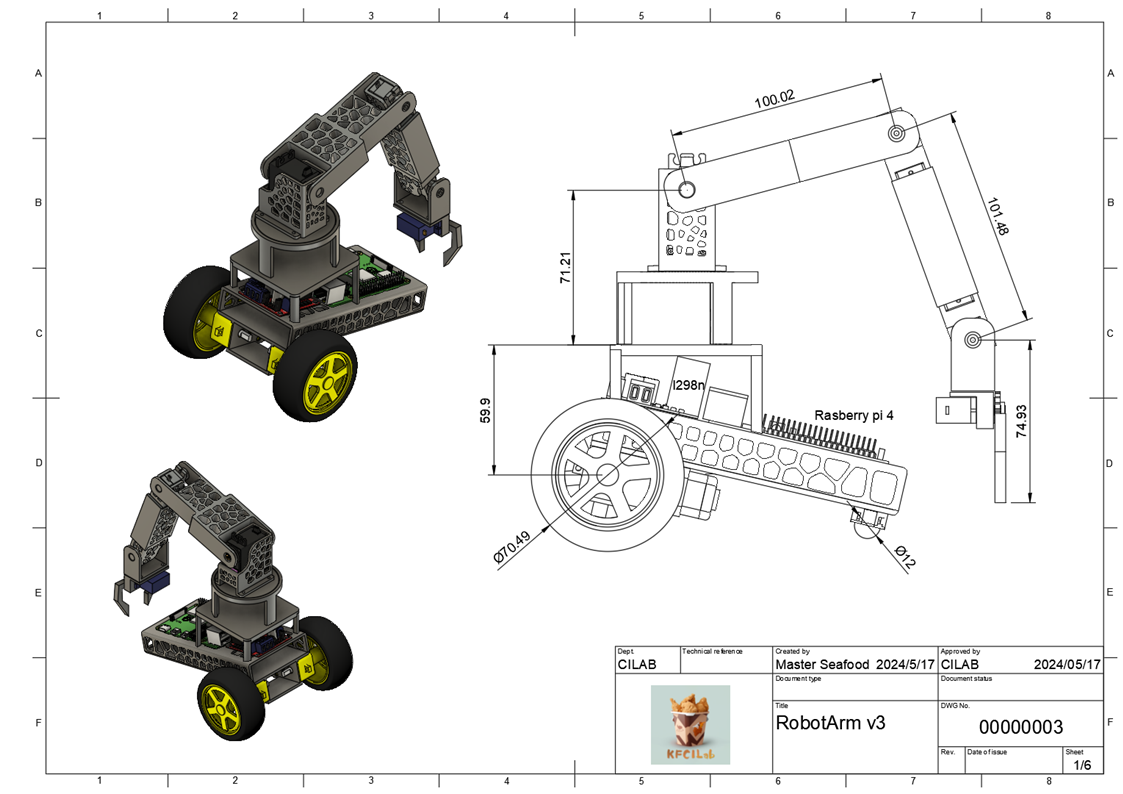
\includegraphics[width=0.9\textwidth]{figures/Armv3 (1).PNG}
    \caption{機械臂版本三設計圖紙 第一頁(單位:mm)}
    %\label{fig:Armv1Drawing_p1}}
\end{figure}

\begin{figure}[htbp]
    \centering
    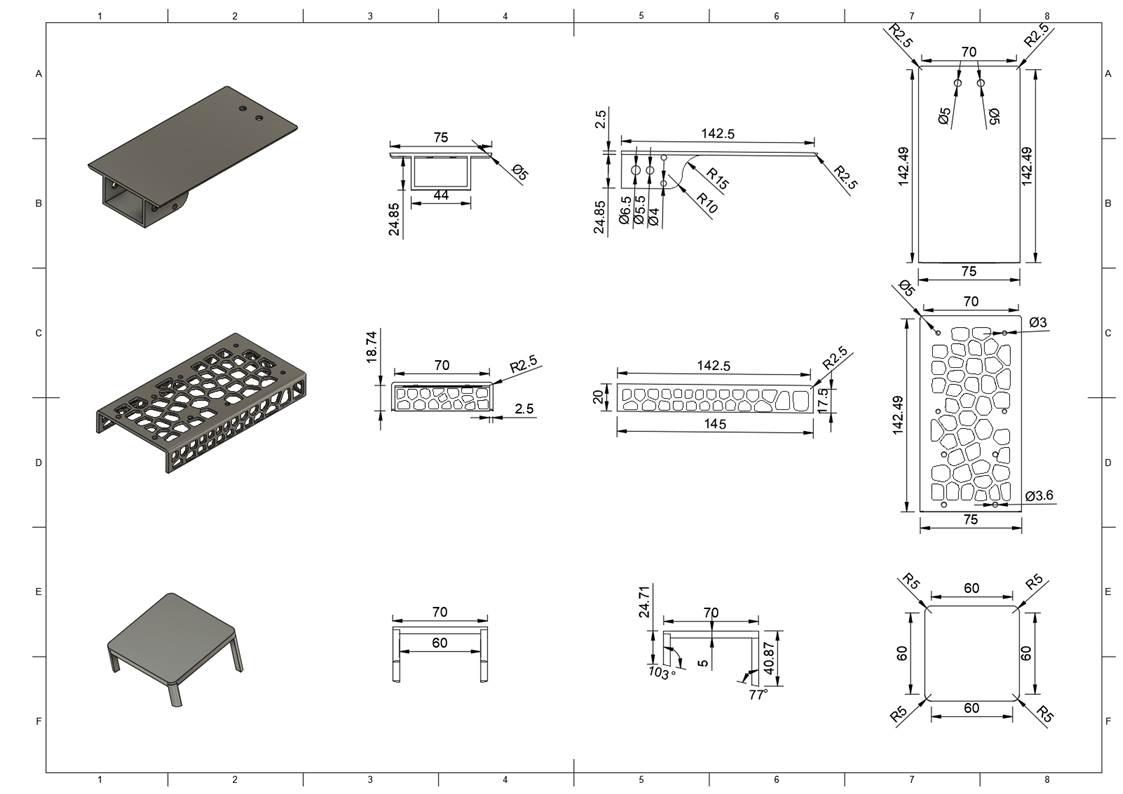
\includegraphics[width=0.9\textwidth]{figures/Armv3 (2).PNG}
    \caption{機械臂版本三設計圖紙 第二頁(單位:mm)}
\end{figure}

\begin{figure}[htbp]
    \centering
    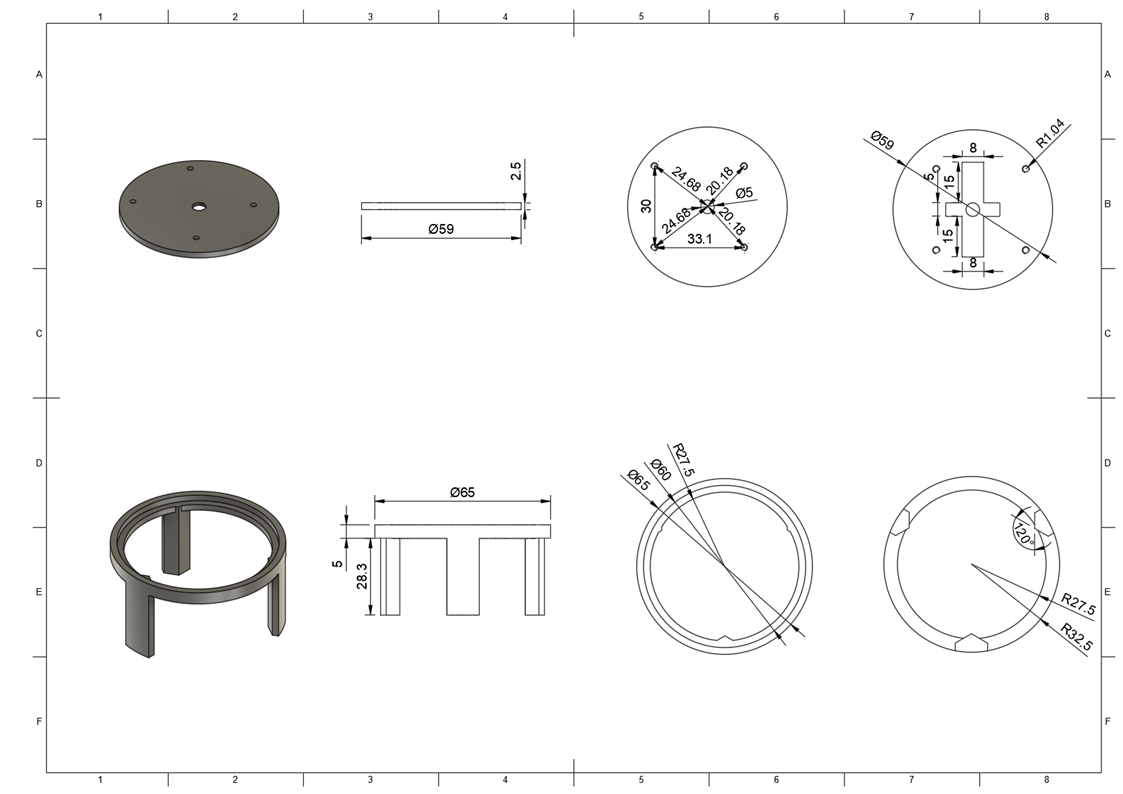
\includegraphics[width=0.9\textwidth]{figures/Armv3 (3).PNG}
    \caption{機械臂版本三設計圖紙 第三頁(單位:mm)}
\end{figure}

\begin{figure}[htbp]
    \centering
    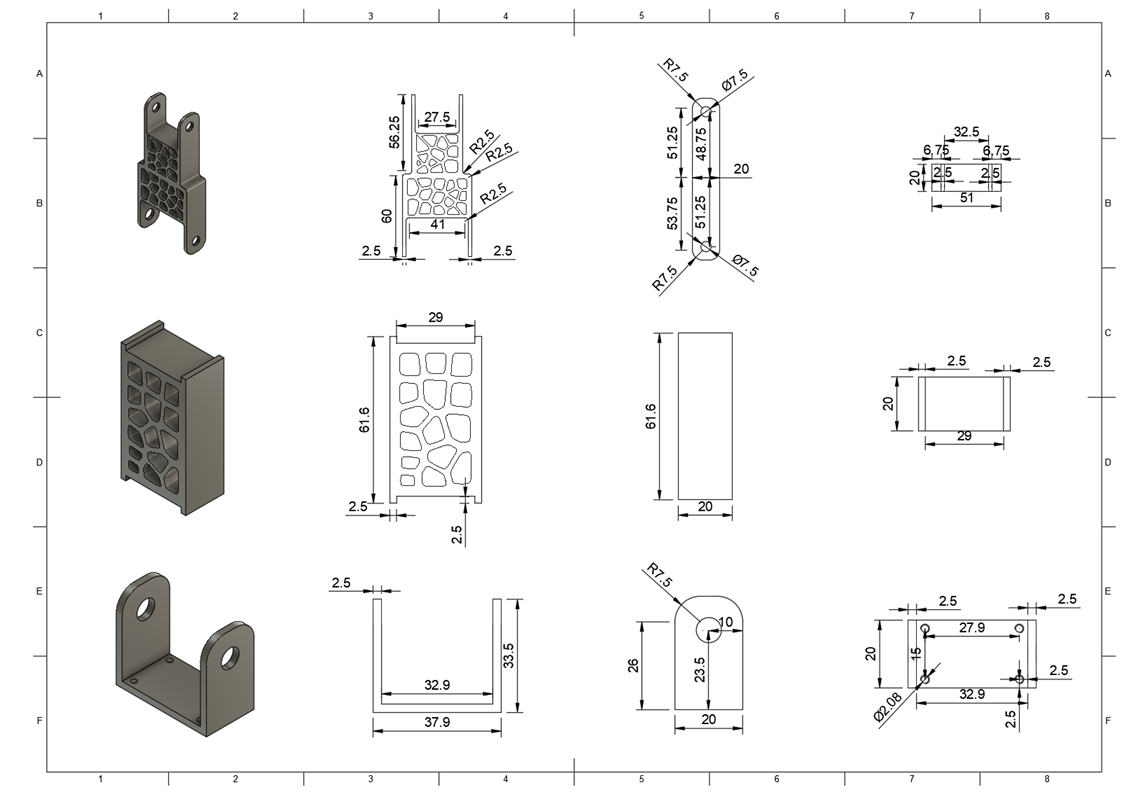
\includegraphics[width=0.9\textwidth]{figures/Armv3 (4).PNG}
    \caption{機械臂版本三設計圖紙 第四頁(單位:mm)}
\end{figure}

\begin{figure}[htbp]
    \centering
    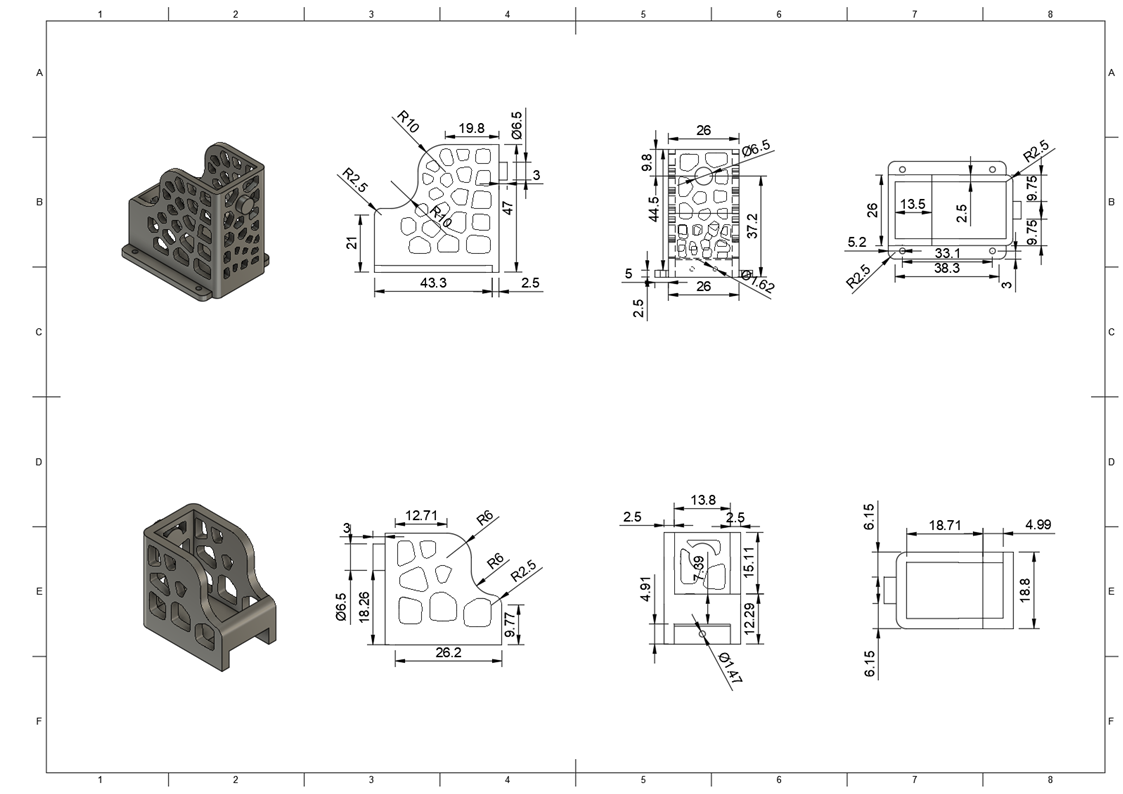
\includegraphics[width=0.9\textwidth]{figures/Armv3 (5).PNG}
    \caption{機械臂版本三設計圖紙 第五頁(單位:mm)}
\end{figure}

\begin{figure}[htbp]
    \centering
    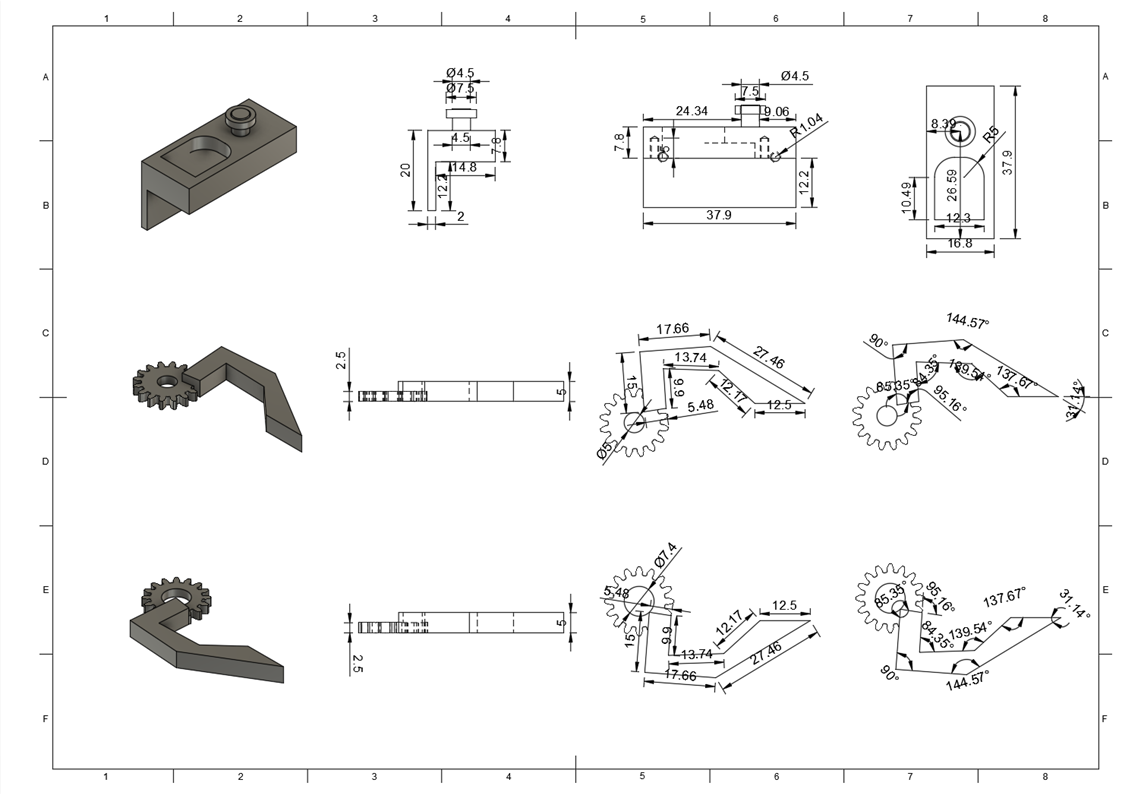
\includegraphics[width=0.9\textwidth]{figures/Armv3 (6).PNG}
    \caption{機械臂版本三設計圖紙 第六頁(單位:mm)}
\end{figure}

\subsection{函數設計}

本實驗將此機器的動作指令簡化為四個函式:

\begin{itemize}
    \item find(color): 配合相機定位,驅動輪子尋找動應顏色的方塊。

    \item aim(color): 配合相機定位,驅動機械臂瞄準對應顏色的方塊。

    \item grab: 驅動機械臂,抓取正下方的物品。

    \item reset: 驅動機械臂,回到初始位置
\end{itemize}

\subsection{下達指令的格式範例}
\begin{listing}
\begin{minted}[frame=single,
               framesep=3mm,
               linenos=true,
               xleftmargin=21pt,
               tabsize=4]{js}
{     
    role: "user",
    content : 
    "The following functions are available:\
    \
    find(color): Let the robot look for a block of a specific color.\
    color option: red, blue.\
    aim(color): Let the robot aim at a block of a specific color.\
    color option: red, blue\
    grab: Make the robot arm grab the block and put it down.\
    reset: Return the robotic arm to its initial position\
    (needs to be executed before each aiming).\
    \
    Please help me use the above functions to control the robot arm,\
    and do not output other text other than the above functions.\
    (Use "," to separate each step)"
},
{
    role: "user", 
    content: "Task: Please grab the red block, and then grab the blue block."
}
\end{minted}
\caption{指令格式範例} 
\end{listing}

\begin{listing}
\begin{minted}[frame=single,
               framesep=3mm,
               linenos=true,
               xleftmargin=21pt,
               tabsize=4]{js}

{
    role="assistant",
    content="find(red), aim(red), grab, reset, find(blue), aim(blue), grab"
}

\end{minted}
\caption{回傳格式範例} 
\end{listing}

\begin{figure}[!hbt]
    %\captionsetup[subfigure]{labelformat=empty} % 完全隱藏圖號
    \centering
    %\subcaptionbox
    %    {初始位置
    %    \label{fig:fig-dataset-contrast-origin}}
    %    {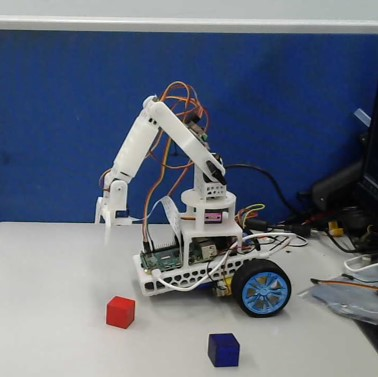
\includegraphics[width=0.4\linewidth]{figures/Exp3 (1)_square.jpg}}
    %~
    \subcaptionbox
        {瞄準紅色方塊
        \label{fig:fig-dataset-contrast-after-adjustment}}
        {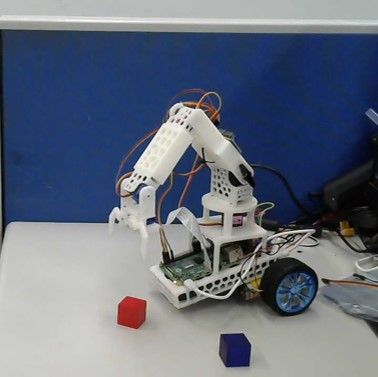
\includegraphics[width=0.4\linewidth]{figures/Exp3 (2)_square.jpg}}
    ~    
    \subcaptionbox
        {夾取紅色方塊
        \label{fig:fig-dataset-contrast-after-adjustment}}
        {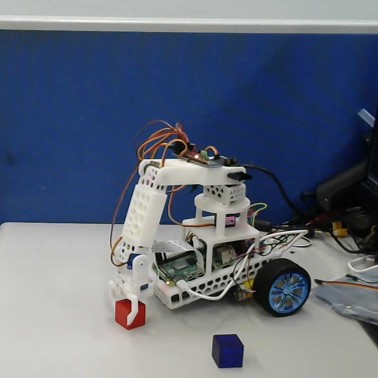
\includegraphics[width=0.4\linewidth]{figures/Exp3 (3)_square.jpg}}
    ~
    \subcaptionbox
        {夾取成功
        \label{fig:fig-dataset-contrast-after-adjustment}}
        {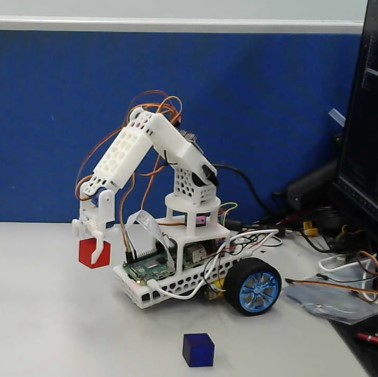
\includegraphics[width=0.4\linewidth]{figures/Exp3 (4)_square.jpg}}
    ~
    \subcaptionbox
        {瞄準藍色方塊
        \label{fig:fig-dataset-contrast-after-adjustment}}
        {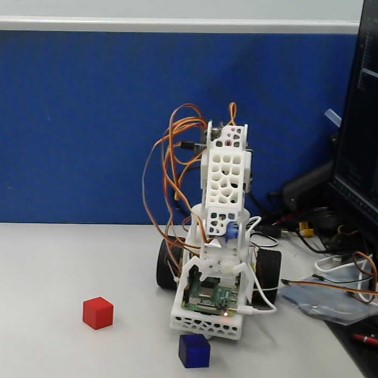
\includegraphics[width=0.4\linewidth]{figures/Exp3 (5)_square.jpg}}
    ~    
    \subcaptionbox
        {夾取藍色方塊
        \label{fig:fig-dataset-contrast-after-adjustment}}
        {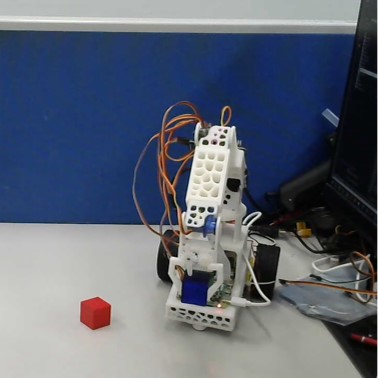
\includegraphics[width=0.4\linewidth]{figures/Exp3 (6)_square.jpg}}
    ~
    \subcaptionbox
        {夾取成功
        \label{fig:fig-dataset-contrast-after-adjustment}}
        {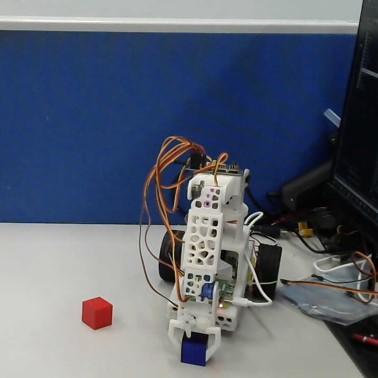
\includegraphics[width=0.4\linewidth]{figures/Exp3 (7)_square.jpg}}   

    \caption{實驗過程縮圖}
\end{figure}


\end{document}